% vim:tw=80:filetype=on:filetype=tex
\subsection{\CChell{} Implementation} \label{sec:system}

\ignore{We implement the prototype of \Chell{} for Linux kernel 3.11
x86-64 with about 7K lines of code.}

The \CChell{} kernel module, \drv{}, manages the system's NVMM memory as a
cache for a conventional file system.  The file system could reside on a disk
or SSD.  \CChell{} must address several challenges to make the cache safe and
efficient.  These include fast cache pages allocation and lookup, efficient
cache eviction and replacement policy, and cache recovery from system failure.
In the following sections we
describe the implementation details about \CChell{}.


\subsubsection{\CChell{} space management}
\label{sec:chellspace}

\ignore{The terminology here is confusing.  There are many btree and Inodes running around.  You need to come up with some names that will make it clear what you are talking about.  For instance maybe Cnode instead of cache Inode.  or CInode or C-Inode.  You also need to name the Btrees.  For instance, one could be the Inode-to-Cnode map or the I2C map.  It'll be clearer to talk about maps rather than Btrees and it makes the discussion more general.  You can just mention that you implement them as btrees.  It sounds as though you basically build a shadow file system that lives in the NVMM and corresponds to the larger file system.  Why not describe it that way?  You could even use it as an organizing idea for the figure.  You could show the big backing store file system and how the NVMM cache file system maps part of it onto NVMM.  Just an idea.}

%\CChell{} is implemented based on the code of PMFS, with many cache related
%new features.

The space allocation and management system in \drv{} is based on PMFS.  It
allocates NVMM in 4~kB pages to minimize fragmentation and wasted space for
small files.  For file systems that store mostly large file, larger 2~MB or
1~GB pages would improve
TLB performance, reduce the number of page faults, and shrink the page table.

\CChell{} uses \emph{cache nodes (Cnode)} to manage cached files.
Cnode is similar to a file system Inode:  It contains the meta information for
the cached contents of a file, including the file size and file access time.
For each file in the backing store device with data in the cache, there is a corresponding
Cnode in \drv{}.
Figure~\ref{fig:CChellspace} shows the data layout of cache space.
The NVMM is divided into three sections: the superblock, the journal area,
and the Cnode and data pages. The superblock
contains information about the cache's layout and is the starting point for crash recovery.

\Drv{} uses two maps to organize the Cnodes and cache pages.
\emph{Inode-to-Cnode~(I2C)} maps Inodes from the backing store to Cnodes in
\CChell{}.  Each Cnode has a map called \emph{Cnode-to-File~(C2F)} that tracks the location
of cached data in NVMM.  Both maps are implemented as B-trees.

When \drv{} starts up, it remaps the whole NVMM region into the kernel's address space. This gives it 
access to superblock region.
The superblock contains a root pointer to the I2C map.
If \drv{} is initialized on an empty
NVMM, it allocates a new I2C map.  If \drv{}
is loaded to recover a existing \CChell{} system, the superblock uses the root
pointer to find the root of the I2C map.

\Drv{} creates an entry in the I2C map on demand for each file that an
application accesses.  The newly-added Cnode contains a pointer to the Cnode's
C2F map, and \drv{} populates it as it brings data for the file into the cache.

\ignore{
\begin{figure}
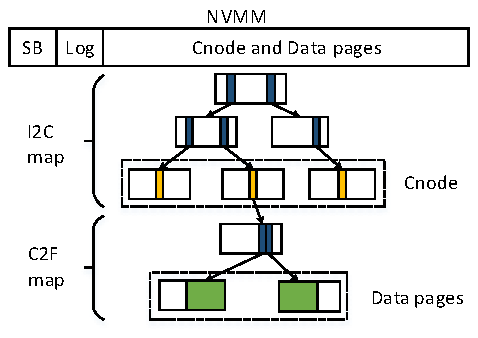
\includegraphics{Figures/Chell-Space.pdf}
\caption{\CChell{} space layout}
\label{fig:CChellspace}
\end{figure}
}

\cfigure[Figures/Chell-Space.pdf,{\figtitle{\CChell{} space layout: \Drv{} uses
two maps to manage NVMM space: Inode-to-Cnode map and Cnode-to-File map
}},fig:CChellspace]

\subsubsection{Cache mmap policy}
\label{sec:mmap}

\ignore{Talk about Chell mmap design options, including: 1. The mmap() size;
2. The MAP\_POPULATE option to reduce the page fault number.
Both two affect the Chell performance. Also the fallocate thing.}

To efficiently perform \texttt{mmap()} operations,
\CChell{} registers a page fault handler to
translate a virtual address to a physical address in NVMM cache.

When a page fault occurs, the OS virtual memory manager (VMM) triggers the
handler, and the handler returns the corresponding cache page
to the VMM, so that the cache page will be mapped directly to the application's
address space.  This avoids the overhead of the page cache and the block layer
for normal \texttt{mmap()} operations and eliminates a \texttt{memcpy()} in \drv{}.
Like \DAChell{}, \CChell{} divides the cached file into 2~MB chunks and
\texttt{mmap()} with 2~MB granularity.

\ignore{Is the following safe?  What happens if someone else is trying to append to the file without going through \drv{}?  is that even allowed?  Does \drv{} interpose on all accesses even if they don't use libchell?  We should definitely mention that.}

If the application appends a file, \CChell{}
need to send the request to the backing store device since the request changes
the metadata. However, if the append size is large (over 32~kB),
\CChell{} does not send the write request to the backing store device directly,
instead it issues a \texttt{fallocate()} to the file system on the backing
store, so the file system will allocate disk space for the append data.  If the \texttt{fallocate()}
succeeds, \CChell{} simply writes the request data to the cache pages
in NVMM, eliminating the overhead to write to backing store device. This requires
the file system on the backing store device to support \texttt{fallocate()},
but the major Linux file systems (e.g., ext4, btrfs~\cite{btrfs}, and xfs~\cite{xfs}) support it.
The append size threshold also affects the performance, as for small
requests, the overhead of \texttt{write()} is smaller than \texttt{fallocate()}.
We show the impact of \texttt{fallocate()} threshold in Section
\ref{sec:microbenchmark}.

\subsubsection{Cache eviction}
\label{sec:evict}

When the cache is full, \drv{} must evict some cache pages to make room for new requests.
Since cache pages may be shared and \texttt{mmap()}ed
to
multiple applications' address spaces, it is essential to remove all the
old mappings of these cache pages before filling them with new data:
otherwise the applications will access invalid or protected data.  \Drv{} removes the
mappings from all the applications' address spaces and then writes back the
data to the backing store device if the cache page is dirty.

\Lib{} does not know whether a cache page has been evicted or not. 
If \lib{} performs a \texttt{memcpy()} on an evicted cache page where the mapping has
been removed, a segmentation fault will occur.  To deal with this situation,
\lib{} installs a signal handler to intercept and handle the segmentation faults.  Upon receiving a SIGSEGV
signal from the handler, \lib{} removes missing memory region 
from its B-tree and tries again. The access will miss, and control will pass to \drv{}. 

\subsubsection{Replacement policy}
\label{sec:replacement}

\Drv{} decides
which Cnode will serve as the victim when an eviction is necesssary.
\drv{} uses
an approximate LRU policy to select the victim.

\drv{} maintains a linked list of Cnodes to track LRU information.
Whenever \drv{} accesses an Cnode, 
\drv{} moves the Cnode to the tail of the list.
During an eviction \drv{} chooses the head of the list.

The LRU information is imperfect, because \drv{} is unaware of many 
accesses to the cached data, since \lib{} accesses the NVMM directly on cache hits.
Since we managed the LRU list as a queue, the result is a blend of LRU and FIFO.
%\andiry{There are several interesting ways to do this:  you could leverage the virtual memory system's clock algorithm to track accesses, or you could periodically mark pages near the head of the LRU list an not accessible.}

%As a result, the head Cnode in the LRU Cnode list may not be the actual least
%recently accessed Cnode from \lib{}.  We may explore the strict LRU replacement
%policy in future work.  

\subsubsection{Dirty data tracking}
\label{sec:dirty}

\CChell{} is a write-back cache, so when \drv{} evicts cache pages, it must know
which data in the cache is dirty, so it can write it back correctly.
Since \lib{} writes to memory mapped cache pages
directly from user space, \drv{} cannot detect changes to the cached data on its own.
Fortunately, the OS already tracks dirty virtual memory
pages: when a memory page is written, the hardware set the dirty bit in the 
page table entry (PTE) of the page, and \CChell{} leverages this facility.
Before evicting a cache page,
\drv{} looks up the page table entry (PTE) in all the mappings of the page.  If
the PTEs has its dirty bit set, \drv{} will write the cache page back to backing store.


\subsubsection{Consistency and recovery}
\label{sec:consistency}

\ignore{This description doesn't make much sense.  You seem to be using undo logging for consistency, but then it sounds like you logically commit the change by writing to the log region.  That sounds like redo logging.  You need to make it more clear how this works, when commit occurs, and how roll back works.  It probably would be better to merge this section with the recovery section, since they are very closely related.}

\CChell{} uses undo logging to ensure that the cache metadata remains
consistent in the event of a crash.  Whenever \drv{} needs to make
a change to a Cnode, allocate a Cnode, or re-allocate pages,
\drv{} records the data in the log and makes it persistent before writing
the new data in place.

Every metadata change is organized as a transaction.  \Drv{} starts
a transaction by allocating the required number of log entries in the journal.
Then, \drv{} fills the log entries with old metadata.
Each log entry is written to the journal and made persistent by flushing it
to NVMM before new data is written in-place.
After all the updates are finished, \drv{} commits the transaction
by writing a special ``finish'' log entry to the journal to invalidate the undo information.

\ignore{Whenever there is change to cache metadata, like cached
file size change or new space allocation,
\drv{} first saves the old value of metadata by writing
logs into the log area, then write the new values in space.}


%\cfigure[Figures/blank.pdf,{\figtitle{\Chell{} space management}:
%A graph shows how \Chell{} managed cache space.},fig:bankshotspace]

If there is a power failure or system crashes, \drv{} can recover the cache
when the system reboots.  During recovery, \drv{} locates the log area using the superblock,
identifies uncommitted transactions and applies the undo information in the log to restore the metadata.
After all the uncommitted transactions have been undone, \CChell{} is in a consistent state.
